% flashcards-title: A door and its scale drawing with dimension arrows
% flashcards-desc: A tall rectangle representing a door, with a small circle for its handle, marked by dimension arrows as two hundred centimeters tall and eighty centimeters wide. Beside it stands a much smaller rectangle of the same shape labeled scale drawing, marked as ten centimeters tall, with its width marked by a question mark. A note says the artwork itself is not drawn to scale.
\documentclass[dvisvgm,tikz,border=8pt]{standalone}
\usepackage{tikz}
\usetikzlibrary{arrows.meta,calc,positioning}
\definecolor{DeckInk}{HTML}{172A3A}
\definecolor{DeckAccent}{HTML}{176B87}
\definecolor{DeckWarm}{HTML}{D97706}
\definecolor{DeckMuted}{HTML}{667784}
\definecolor{DeckPaper}{HTML}{F7FAFC}
\tikzset{
  every node/.style={font=\sffamily, text=DeckInk},
  object/.style={draw=DeckInk, line width=1.1pt, fill=DeckPaper},
  primary/.style={draw=DeckAccent, line width=1.5pt},
  boundary/.style={draw=DeckAccent, line width=1.5pt, dashed, rounded corners=6pt},
  guide/.style={draw=DeckMuted, line width=0.9pt, dashed},
  dimension/.style={{Stealth[length=3.2mm,width=2.2mm]}-{Stealth[length=3.2mm,width=2.2mm]}, draw=DeckWarm, line width=1.2pt},
  motion/.style={-{Stealth[length=3.5mm,width=2.5mm]}, draw=DeckAccent, line width=1.5pt, dashed},
}

\begin{document}
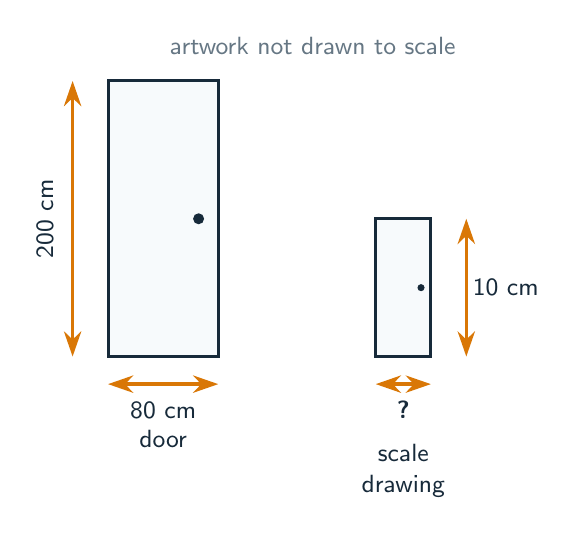
\begin{tikzpicture}[x=1cm,y=1cm]
  % Real door (aspect 80 : 200 = 0.4)
  \draw[object] (0,0) rectangle (1.4,3.5);
  \fill[DeckInk] (1.15,1.75) circle (0.07);
  \node[font=\sffamily\small] at (0.7,-1.05) {door};
  \draw[dimension] (-0.45,0) -- (-0.45,3.5);
  \node[font=\sffamily\small, rotate=90] at (-0.8,1.75) {200 cm};
  \draw[dimension] (0,-0.35) -- (1.4,-0.35);
  \node[font=\sffamily\small] at (0.7,-0.68) {80 cm};
  % Scale drawing (same aspect, smaller)
  \begin{scope}[xshift=3.4cm,yshift=0cm]
    \draw[object] (0,0) rectangle (0.7,1.75);
    \fill[DeckInk] (0.575,0.875) circle (0.045);
    \node[font=\sffamily\small, align=center] at (0.35,-1.45) {scale\\drawing};
    \draw[dimension] (1.15,0) -- (1.15,1.75);
    \node[font=\sffamily\small] at (1.65,0.875) {10 cm};
    \draw[dimension] (0,-0.35) -- (0.7,-0.35);
    \node[font=\sffamily\small\bfseries] at (0.35,-0.68) {?};
  \end{scope}
  \node[font=\sffamily\small, text=DeckMuted] at (2.6,3.95) {artwork not drawn to scale};
\end{tikzpicture}
\end{document}
